\chapter{Vaman Based Applications}

\section{UGV (Unmanned Ground Vehicle)}

\subsection{Navigation using Fly-sky Transmitter and Receiver} 
\subsubsection{Required components/Software tools}
\begin{itemize}
    \item  UGV chassis with DC motors
    \item  Vaman micro-controller with Type-B USB cable
    \item  L293D Motor Driver IC
    \item  Fly-sky Transmitter and Receiver
    \item  Breadboard
    \item  Jumper Wires
    \item  QORC SDK installed on linux system with supporting tools.
\end{itemize}

\subsubsection{Steps}
\begin{itemize}
    \item Make the connections as per the wiring diagram (Figure \ref{Wiring_UGV_flysky_Vaman}).
    \item Connect the Vaman board to Laptop/PC using Type-B USB cable.
    \item Run ”make” command in ”GCC project” folder to generate bin file for the ”main.c” file at the code link at (\ref{Code_link_UGV_flysky_vaman})
    \item Flash the generated bin file on Vaman using the tinyfpga-programmer-gui.py tool.
    \item Test whether the UGV is navigating as per the command sent from the transmitter.
\end{itemize}

\subsubsection{Code link} \label{Code_link_UGV_flysky_vaman}
\begin{tcolorbox}
\url{https://github.com/sachinomdubey/Projects/tree/main/Autonomous\%20Navigation/UGV/Vaman/Vaman_UGV_flysky/src}
\end{tcolorbox}

\begin{figure}[h!]
\centering
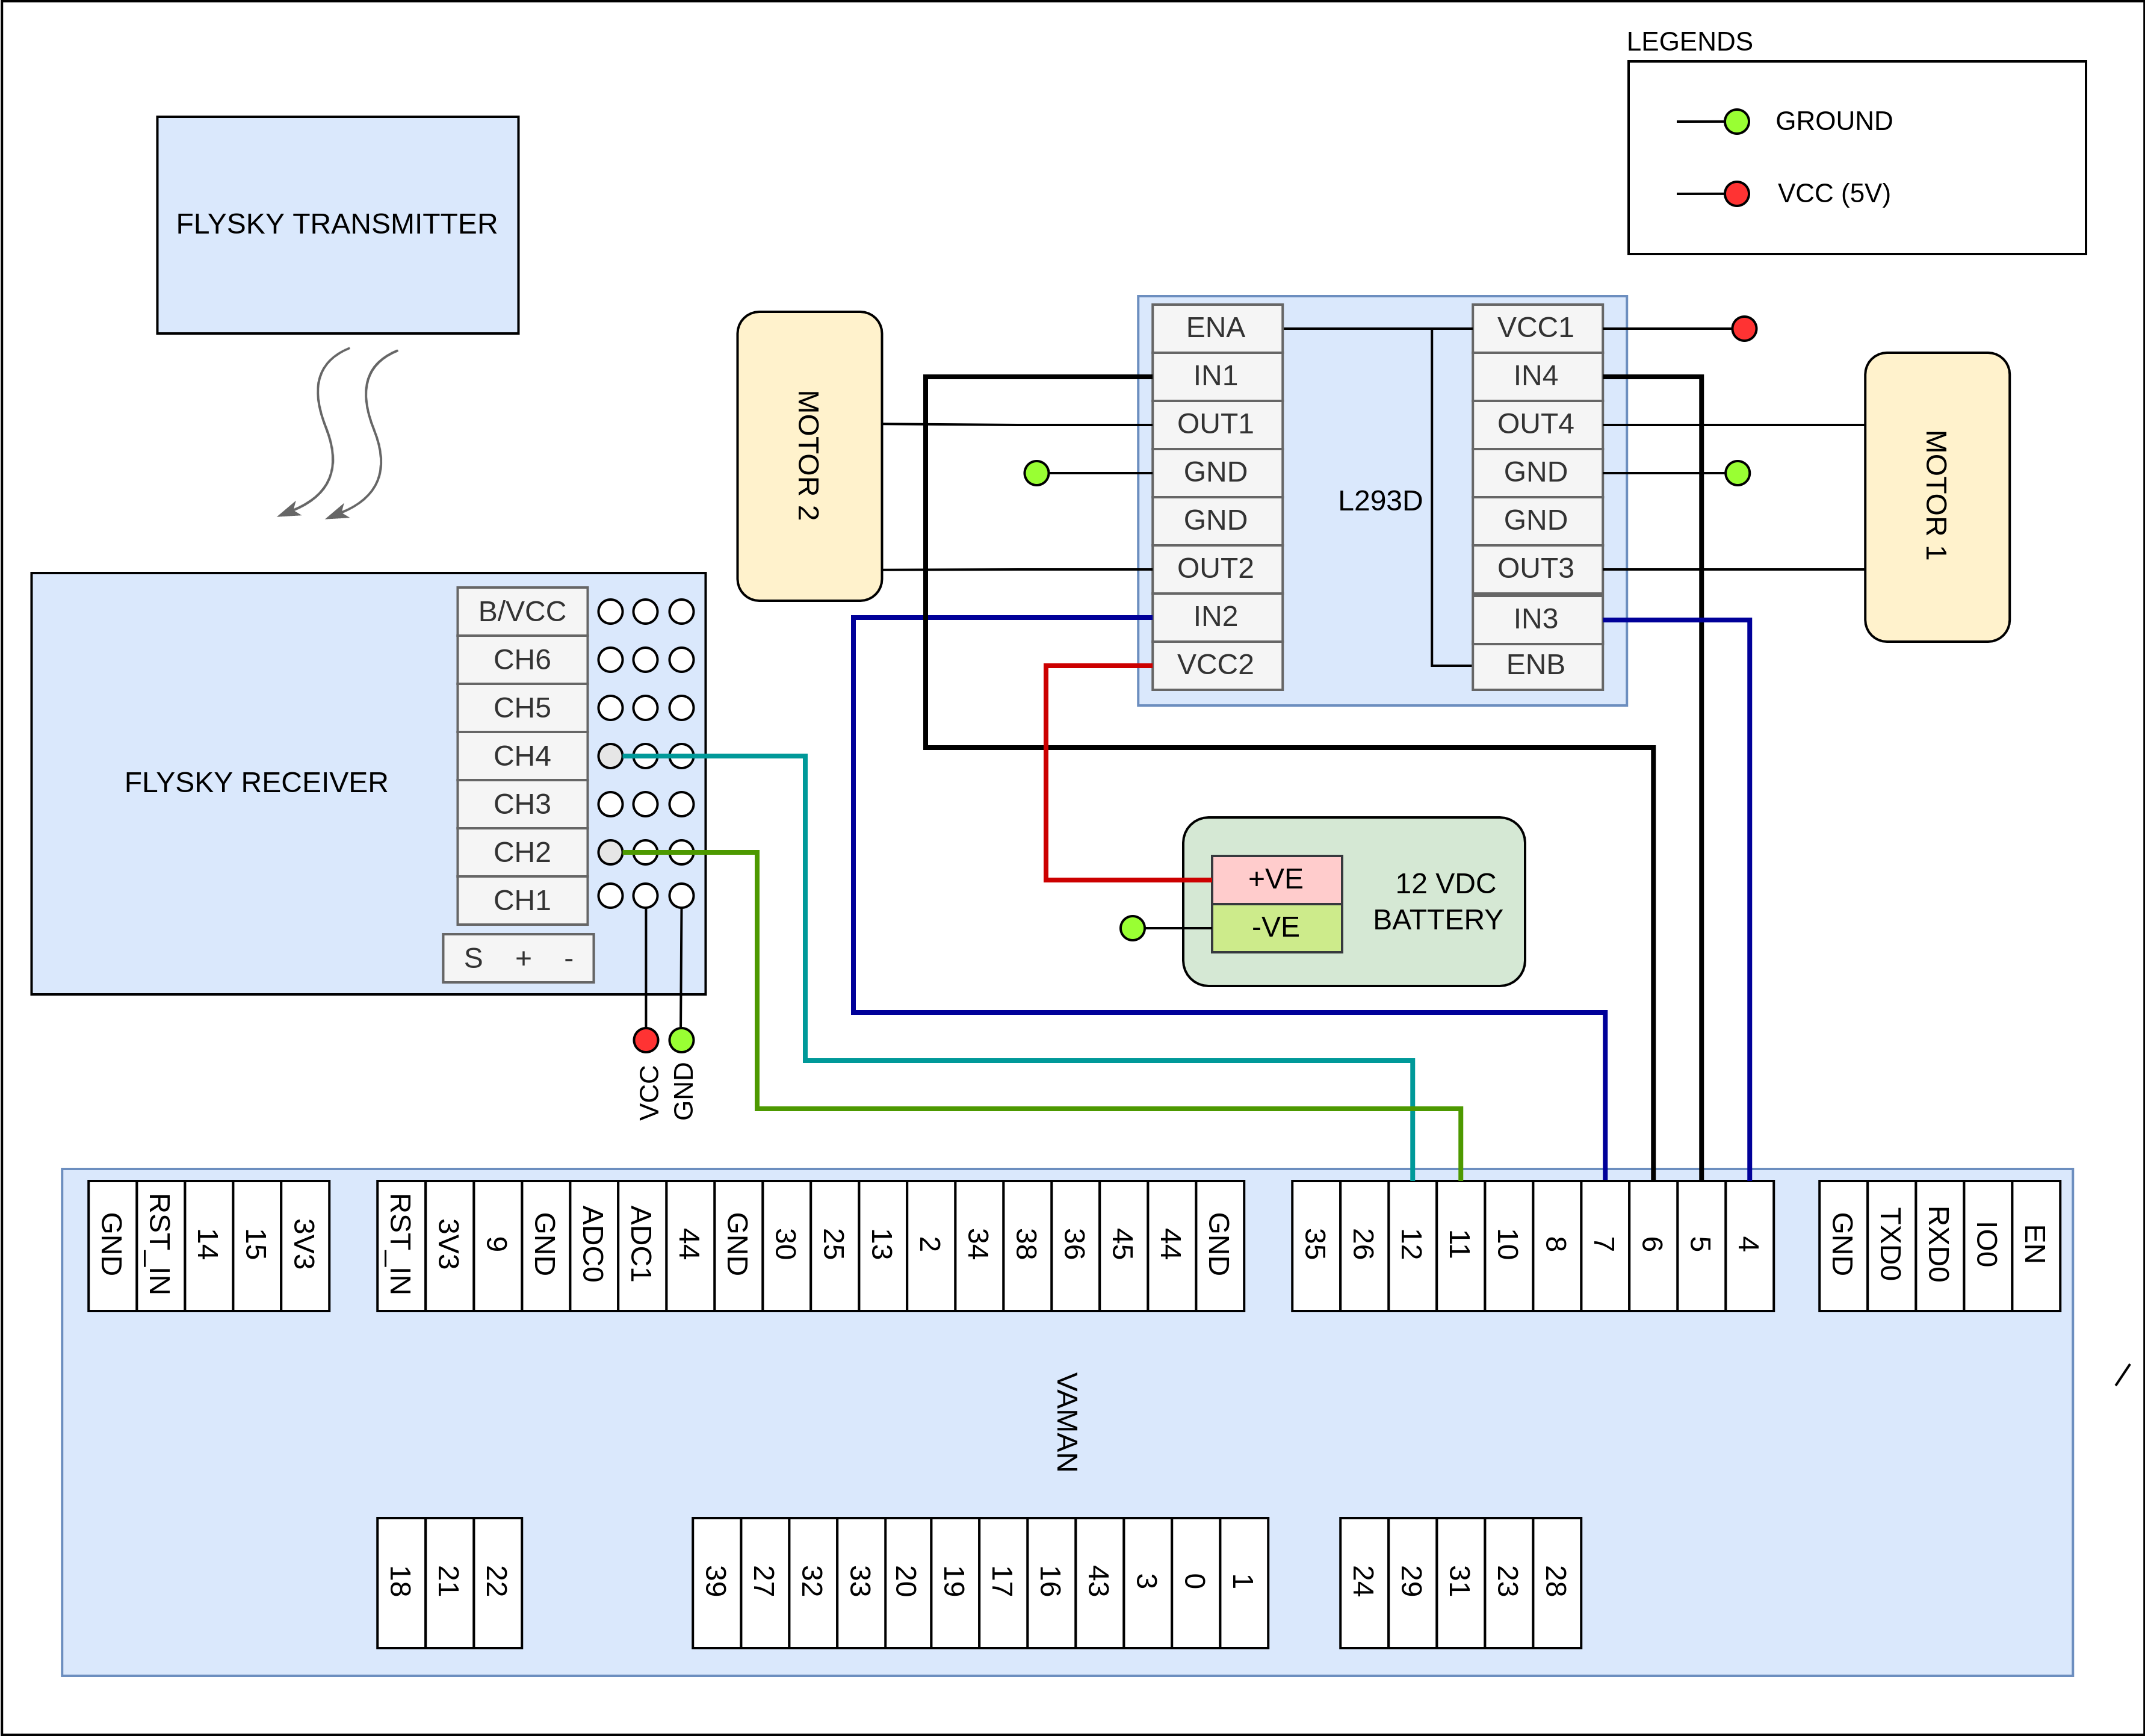
\includegraphics[width=\columnwidth]{./Figures/Wiring_UGV_flysky_Vaman.png}
\caption{Wiring Diagram for UGV Navigation using Fly-sky transmitter \& receiver (Vaman)}
\label{Wiring_UGV_flysky_Vaman}
\end{figure}

\subsubsection{Working}
\begin{itemize}
    \item User first give navigation input using the Throttle and Roll sticks on transmitter. This input is transmitted to the receiver wirelessly.
    \item Receiver generates PWM signals on channel-2 and channel-4 as per the navigation input received from the transmitter.
    \item These PWM signals are read by the Vaman using pulseIn function.
    \item Depending on the read values the C program sends suitable commands (forward, backward, left, right and stop) to the direction control pins of Motor driver IC.
\end{itemize}

\subsection{Navigation using Android phone} 
\subsubsection{Required components/Software tools}
\begin{itemize}
    \item  UGV chassis with DC motors
    \item  Vaman development board with type-B USB cable
    \item  L293D Motor Driver IC
    \item  Breadboard
    \item  Jumper Wires
    \item  QORC SDK installed on linux system with supporting tools
    \item  Android phone with Dabble app installed.
\end{itemize}



\subsubsection{Steps}
\begin{itemize}
    \item Make the connections as per the wiring diagram (Figure \ref{Wiring_UGV_phone_vaman}).
    \item Connect the Vaman board to Laptop/PC using Type-B USB cable.
    \item Run "make" command in "GCC\_project" folder to generate bin file for the "main.c" file at the code link (\ref{Code_link_UGV_phone_vaman}).
    \item Flash the generated bin file on Vaman using the tinyfpga-programmer-gui.py tool. 
    \item Verify that the UGV navigates as per the command received from dabble app installed on the android phone.
\end{itemize}

\subsubsection{{Code link}}\label{Code_link_UGV_phone_vaman}
\begin{tcolorbox}
\url{https://github.com/sachinomdubey/Projects/tree/main/Autonomous\%20Navigation/UGV/Vaman/Vaman_mobile_control/src}
\end{tcolorbox}

\begin{figure}[h!]
\centering
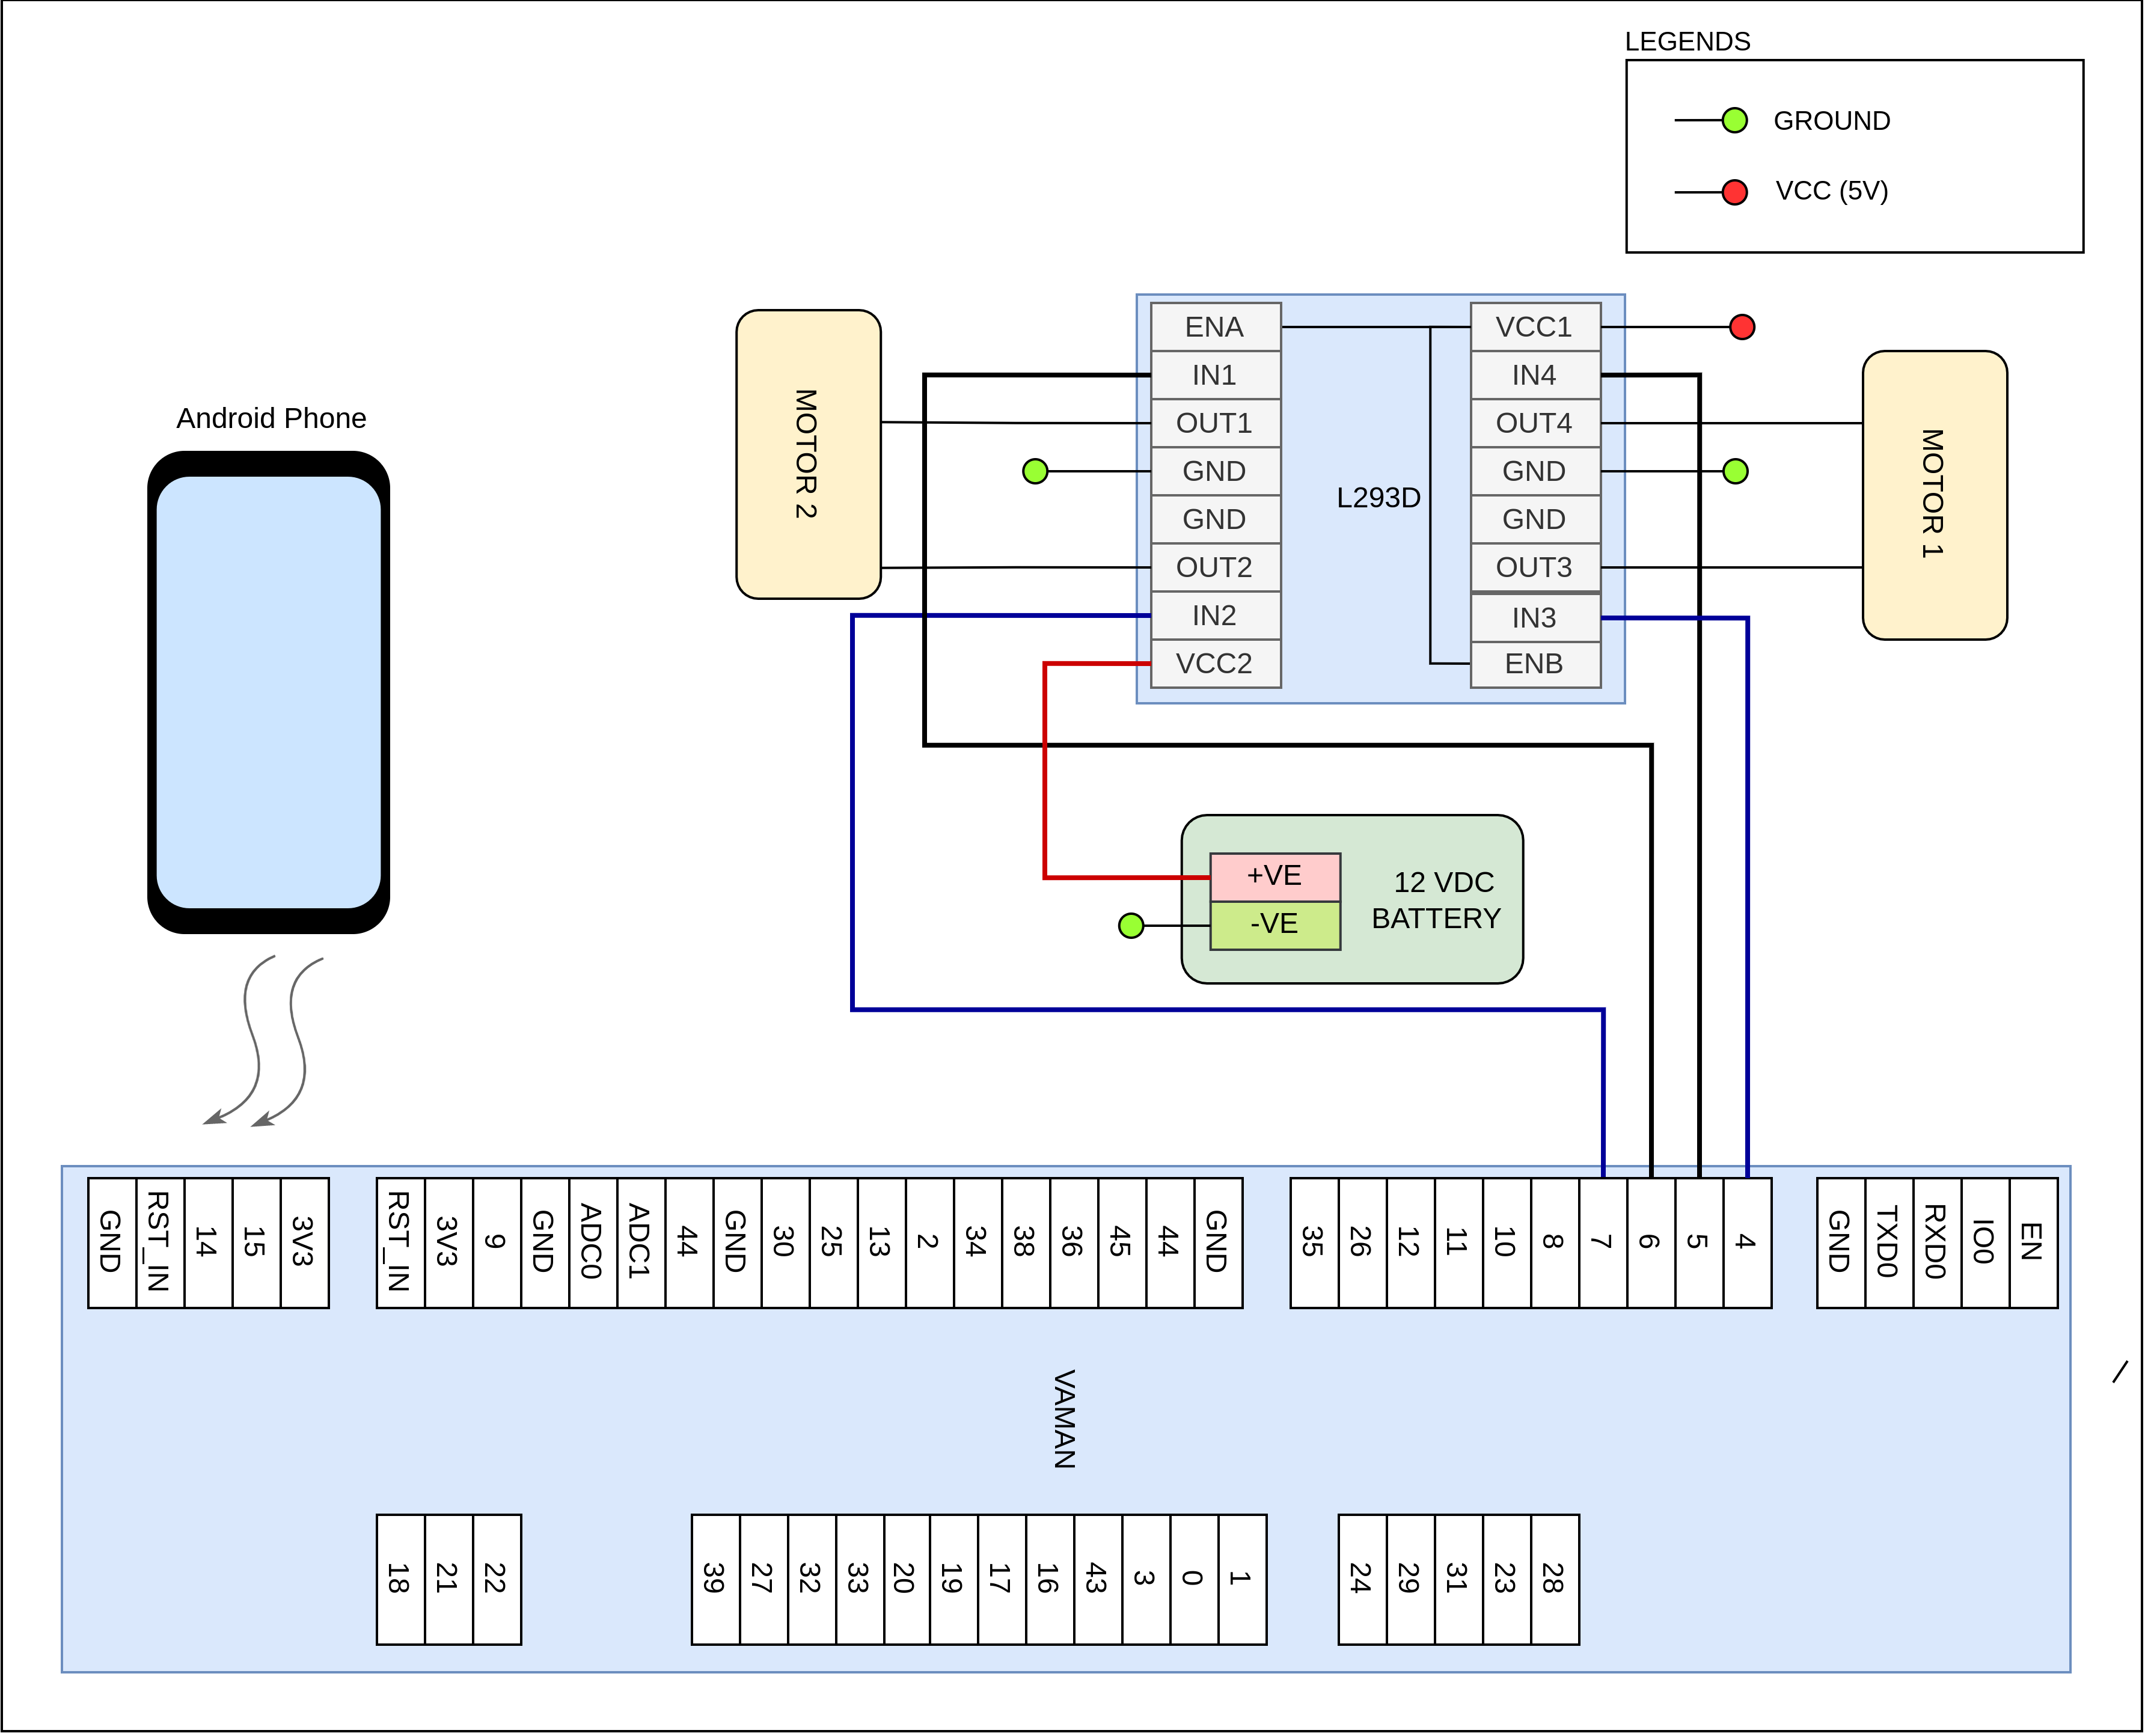
\includegraphics[width=\columnwidth]{./Figures/Wiring_UGV_phone_vaman.png}
\caption{Wiring Diagram for UGV Navigation using Android phone (Vaman)}
\label{Wiring_UGV_phone_vaman}
\end{figure}

\subsubsection{Working}
\begin{itemize}
    \item User gives navigation input using the dabble app installed on the android device. The dabble app communicates to Vaman over bluetooth. The dabble app UI is as shown in figure \ref{Dabble_app_UI}.
    \item Depending on the input received over bluetooth, the program sends suitable commands (forward, backward, left, right and stop) to the direction control pins of Motor driver IC.
\end{itemize}

\newpage
\section{Simultaneous execution of tasks using FreeRTOS}

Embedded systems uses real-time operating system. Real-time tasks are critical as timing places an important role in such systems. RTOS are made to run tasks or program with precise timings and high degree of reliability. It helps in multitasking even when the micro-controller unit has a single core to execute these tasks.

FreeRTOS is an open source RTOS which are designed, but not limited to run on small micro-controllers (8/16 bit). With basic knowledge of RTOS, we can use FreeRTOS as there is a lot of documentation available for it.

In this program, we have run two different tasks in parallel on Vaman using FreeRTOS. The two tasks are as follow:
\begin{enumerate}
    \item Blinking LED connected at pin 13 of Arduino.
    \item Speeding up and slowing down a DC motor continuously in a loop.
\end{enumerate}

\subsubsection{Required components/Software tools}
\begin{itemize}
    \item Vaman (pygmy BB4) development board
    \item LED connected between pin 12 of Vaman and GND.
    \item L293D motor driver IC
    \item 12V DC Battery for motor
    \item Type-B cable for powering and programming Vaman
    \item Jumper Wires
    \item QORC SDK installed on the Linux system along with required support tools.
\end{itemize}

\begin{figure}[ht]
\centering
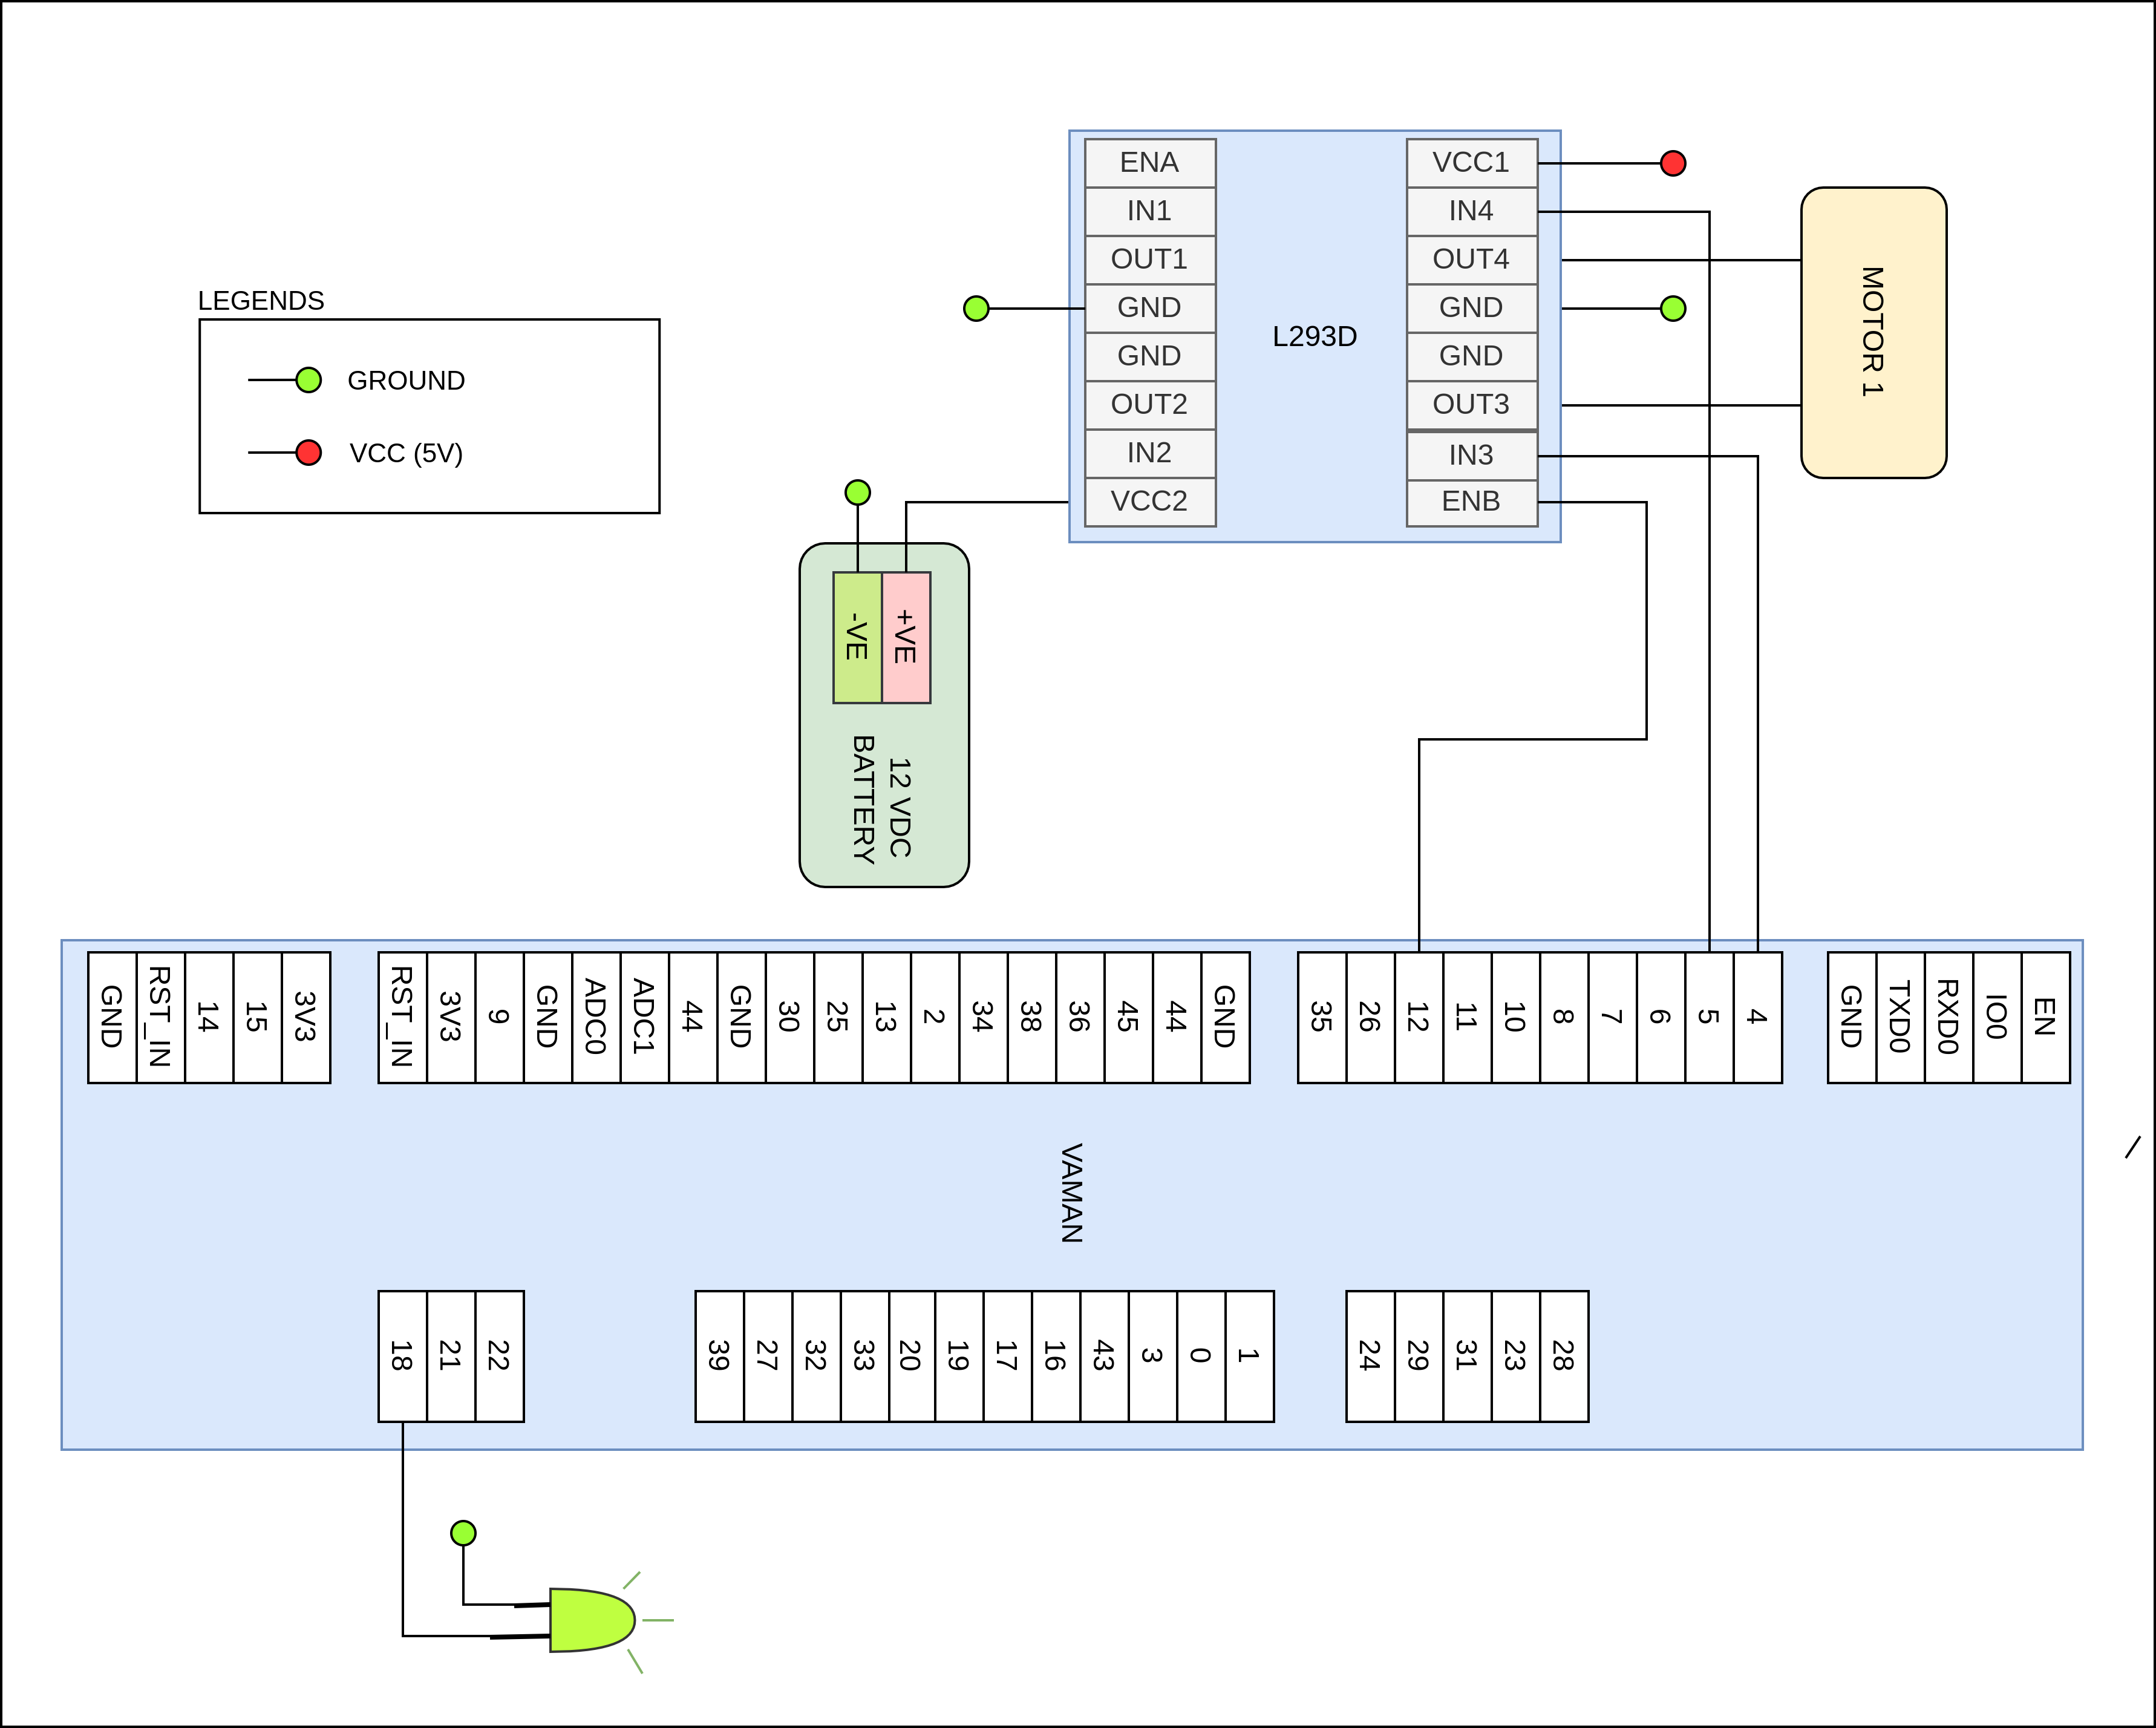
\includegraphics[width=\columnwidth]{./Figures/Wiring_FreeRTOS_demo_vaman.png}
\caption{Wiring diagram for running two tasks simultaneously on Vaman.}
\label{Wiring_FreeRTOS_demo_vaman}
\end{figure}

\subsubsection{Steps}
\begin{itemize}
    \item Make the connections as per the wiring diagram (Figure \ref{Wiring_FreeRTOS_demo_vaman}).
    \item Connect the Vaman board to Laptop/PC using Type-B USB cable.
    \item Run "make" command in "GCC\_project" folder to generate bin file for the "main.c" file at the code link (\ref{Code_link_FreeRTOS_Vaman}).
    \item Flash the generated bin file on Vaman using the tinyfpga-programmer-gui.py tool. 
    \item Verify that the LED blinks and the motor also changes speed simultaneously.
\end{itemize}

\subsubsection{Code link} \label{Code_link_FreeRTOS_Vaman}
\begin{tcolorbox}
\url{https://github.com/sachinomdubey/Projects/tree/main/Autonomous\%20Navigation/FreeRTOS/Vaman_Blink_MotorControl/src}
\end{tcolorbox}

\subsubsection{Working}
\begin{itemize}
    \item First the FreeRTOS library is included using the below line. This header contains all the functions required to create, schedule and run tasks in parallel.
    \begin{lstlisting}[language=C]
    #include <FreeRTOS.h>
    \end{lstlisting}
    \item For creating task, \textbf{xTaskCreate()} API is called in setup function with certain parameters/arguments.
    \begin{lstlisting}[language=C]
    xTaskCreate( TaskFunction_t pvTaskCode, const char * const pcName,
    uint16_t usStackDepth, void *pvParameters, UBaseType_t uxPriority,
    TaskHandle_t *pxCreatedTask );
    \end{lstlisting}
    \item Example of task creation
    \begin{lstlisting}
    xTaskCreate(task1,"task1",128,NULL,1,NULL);
    xTaskCreate(task2,"task2",128,NULL,2,NULL);  
    \end{lstlisting}
    \item After creating the task, start the scheduler in a main function using \textbf{vTaskStartScheduler()} API.
    \item \textbf{main()} function will remain empty as we don’t want to run any task manually and infinitely. Because task execution is now handled by Scheduler.
    \item Next we define our tasks using below format and write logic for it. Everything else is taken by FreeRTOS library function and we can observe the tasks running in parallel on executing the written program.
    \begin{lstlisting}
    void task1(void *pvParameters)  
    {
        while(1) {
            ..
            ..//your logic
        }
    }
    \end{lstlisting}
\end{itemize}
\newpage





